\documentclass{article}

\usepackage[english]{babel}
\usepackage[utf8x]{inputenc}
\usepackage{amsmath}
\usepackage{graphicx}
\usepackage[colorinlistoftodos]{todonotes}
\usepackage{float}
\usepackage[export]{adjustbox}
\usepackage[top=2cm, bottom=2cm, left=2cm, right=2cm]{geometry}

\title{PIC Ebola Outbreak Model}
\author{Chelsea Sandridge, Eric Jones, Kelsey Kalmbach, and Paul Diaz 
\thanks{Colorado School of Mines. Math 484: Capstone. Advisor: Stephen Pankavich}}


\begin{document}
\maketitle 

\section{Assumptions}
\begin{itemize}
\item Infected individuals become either (dead and infectious) or (recovered and removed) from the model (people who recover from the disease are no longer susceptible)
\item Individuals who have died from the disease but who have not yet been buried can still infect susceptible individuals.
\end{itemize}

\section{Our Methods}
Our case data has been extracted from a GitHub repository maintained by Caitlin Rivers \\ (\texttt{https://github.com/cmrivers/ebola}), a graduate student at Virginia Tech. This data includes time-series estimates for the number of cases and deaths in Guinea, Liberia, and Sierra Leone.  
We are then using Matlab's built in solver fminsearch to fit the infection rate parameters $k_1$ and $k_2$ using this data. Furthermore, we assumed constant values for all other parameters which were determined by estimated values for this outbreak. These particular values are detailed further in Section 4.  
\section{Mathematical Model}

\begin{equation} \left\lbrace
\begin{aligned} 
\frac{dS}{dt} &= \alpha S - k_1 S I -k_2 S R_I \\
\frac{dE}{dt} &=  k_1 S I +k_2 S R_I - \mu E \\
\frac{dI}{dt} &=  \mu E - \gamma I\\
\frac{dR_I}{dt} &= \rho\gamma I - \beta R_I \\
\frac{dR_B}{dt} &= \beta R_I \\
\frac{dR_R}{dt} &= (1-\rho)\gamma I \\
\end{aligned} \label{std_seir}
\right.
 \end{equation} \\
 
   
Here $S$ is the susceptible population, $E$ is the exposed population, i.e. those who have the disease but are not yet symptomatic, $I$ is the infectious population, $R_I$ is the removed and infectious population, i.e. those who have died but not yet been buried, $R_B$ is the removed and buried population, and $R_R$ is the removed and recovered population.

\begin{align*}
\alpha &= \text{population growth constant} \\
k_1    &= \text{transmission rate between infected and susceptible} \\
k_2	   &= \text{transmission rate between removed and still infectious and susceptible} \\
\mu    &= \text{rate at which people move from exposed to infected} \\
\gamma &= (\text{average time with disease} )^{-1}\\
\rho   &= \text{the proportion of people who die of the disease} \\
\beta  &= (\text{time until one is buried})^{-1}
\end{align*}

\section{Parameter Values}
\begin{align*}
\alpha &=  \text{known empirically for each of the three countries \cite{WorldBank}}\\
\mu    &= \frac{1}{21 \text{ days}},\ \text{one over the  incubation period of the virus } \cite{CDC2}  \\
\gamma &= \frac{1}{10 \text{ days}},\ \text{one over the average duration of infection } \cite{CDC2} \\ 
\beta  &= \frac{1}{1 \text{ day}}, \ \text{one over the average rate of burial }  \cite{betaTerm} \\ % this source indicated that beta may be slightly different from 1, if we want to change this.
\rho   &= 0.70 \ \text{estimated value from the World Health Organization } \cite{deathRate}
\end{align*}

\section{Next Steps}
We are still working out which parameters would best be fit to our data using fminsearch. We know that $k_1$ and $k_2$ would be best determined in this manner but we might also consider fitting $\beta$, as finding data regarding burials in these countries is not well documented. We would also like to perform sensitivity analysis on some of the parameters. In particular, the known values for $\mu$ and $\gamma$ have a wide range, so it would be useful to know how this uncertainty will effect our model. \\

The data that we are using has ``cases'' and ``deaths'' due to ebola in the countries of Guinea, Sierra Leone, and Liberia. Once we have a consistent fit method that gives realistic result (e.g. finds positive parameter values which fit the data), we will use the same method on each of the three countries. We expect the parameters between countries to be similar but slightly different (from these parameter values, we can potentially judge how ``infectious'' ebola is in one country versus another). Then, we will connect the different countries using compartmental transfer terms (i.e. $\displaystyle \frac{dI_{Liberia}}{dt} = I_{Guinea}\zeta_{LG} + I_{SierraLeone}\zeta_{LS}$, where $\zeta_{i,j}$ are the transfer terms, or something of this sort), and we will fit the three transfer parameters in a similar method as we fit the intranational parameters. \\

Lastly, we will consider what effect a treatment center would have on our model; would it alter $k_1$, or $\mu$, or some other parameter? Once we make this decision, and determine the magnitude of the effect a treatment center would have, we will try putting the center in each of the three countries, and find where the best placement is (where ``best'' will be determined by some cost function we haven't determined yet). \\

Below are two of the figures which we have generated thus far. The first represents our first attempt at fitting $k$ in a non-modified SEIR model to the case data in Liberia. The second is a two parameter fit ($k_1$ and $\beta$) using case data in Guinea and our modified SEIR model. 
With regards to Figure 1, we were not sure if the $k$ value that was being fit was on the right order of magnitude. Our value here was on the order of $10^{-8}$. In Figure 2, there exists a large discrepancy between our data and our models estimate for the removed population. \\

We plan to continue trying different fitting methods, including fitting to the number of deaths rather than the number of cases. We also plan to continue fitting various parameters--- we think $k_1$ is very important to fit to, but are less sure which other parameters are important. A sensitivity analysis will help clear up the most important parameters, and give us some basis for which parameters are the most important to fit.


      \begin{figure}[H]
            	\centering
        		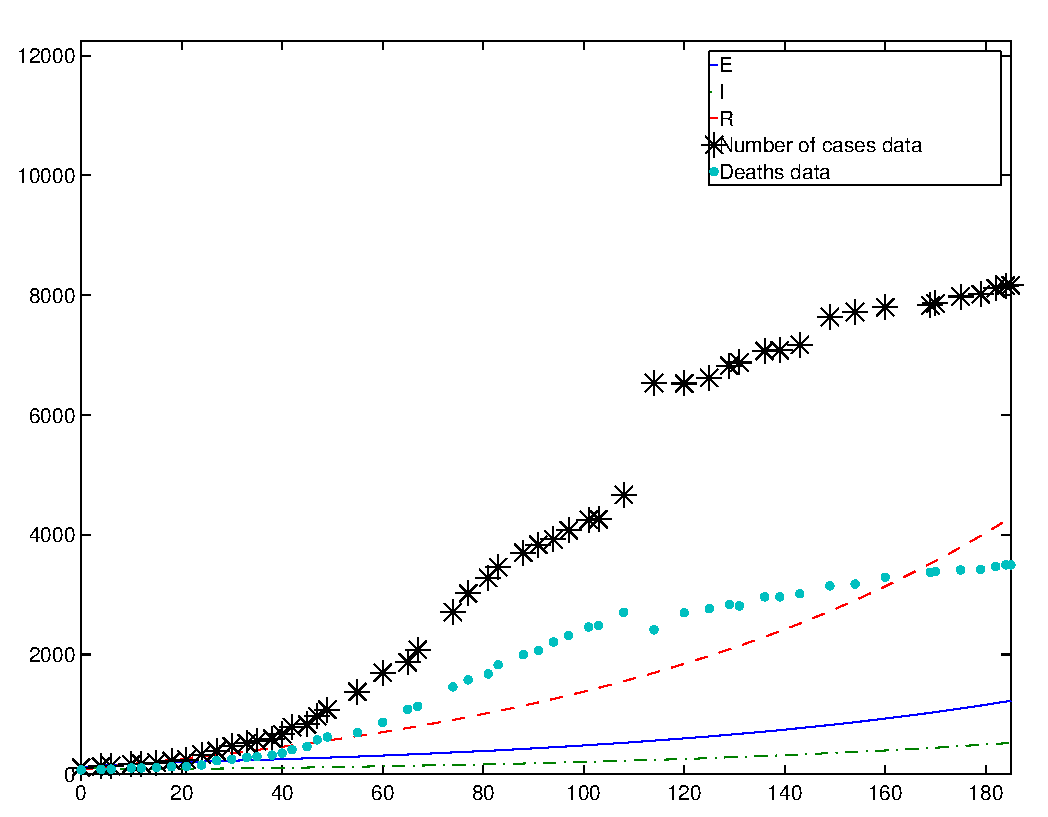
\includegraphics[width =13cm]{seir_model_param_fit.eps}
                \caption{Liberia case data with unmodified SEIR model}
       \end{figure}
            
       \begin{figure}[H]
           	\centering
       		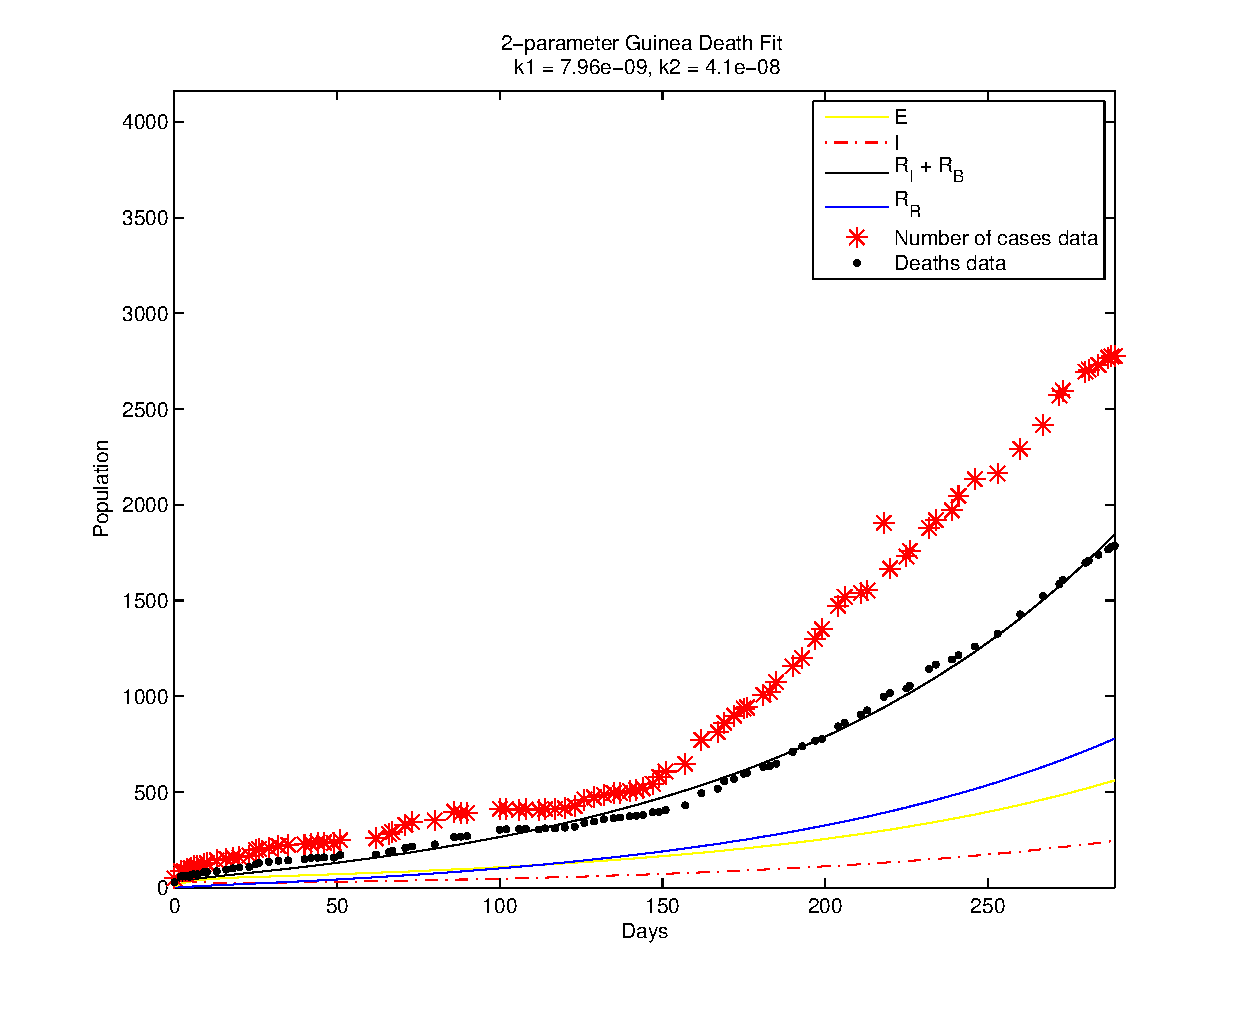
\includegraphics[width =14cm]{guinea2param.eps}
            \caption{Guinea death data with modified SEIR model (Eqn. 1)}
       \end{figure}
       


\begin{thebibliography}{3}

\bibitem{WorldBank} ``Population Growth (annual \%)." The World Bank. Web. 26 Mar. 2015. http://data.worldbank.org/indicator/SP.POP.GROW. 

\bibitem{CDC2} ``Signs and Symptoms." Centers for Disease Control and Prevention. N.p., n.d. Web. 27 Mar. 2015. http://www.cdc.gov/vhf/ebola/symptoms/index.html. 

\bibitem{betaTerm}Nielsen, Carrie F., Sarah Kidd, Ansumana Sillah, Edward Davis, and Jonathan Mermin. ``Improving Burial Practices and Cemetery Management During an Ebola Virus Disease Epidemic — Sierra Leone, 2014." Centers for Disease Control and Prevention. \emph{Centers for Disease Control and Prevention,} 16 Jan. 2015. Web. 26 Mar. 2015.

\bibitem{deathRate} Epatko, Larisa. ``70 percent Ebola death rate? Here’s how they calculate it." \emph{PBS News Hours.} N.p., 16 Oct. 2014. Web. 26 Mar. 2015. http://www.pbs.org/newshour/rundown/70-percent-ebola-death-rate-calculate/. 



\end{thebibliography}	
                                                                         
\end{document}